\documentclass{article}

\usepackage{tikz}
\usepackage[inner=0.5cm,outer=0.5cm]{geometry}

\begin{document}

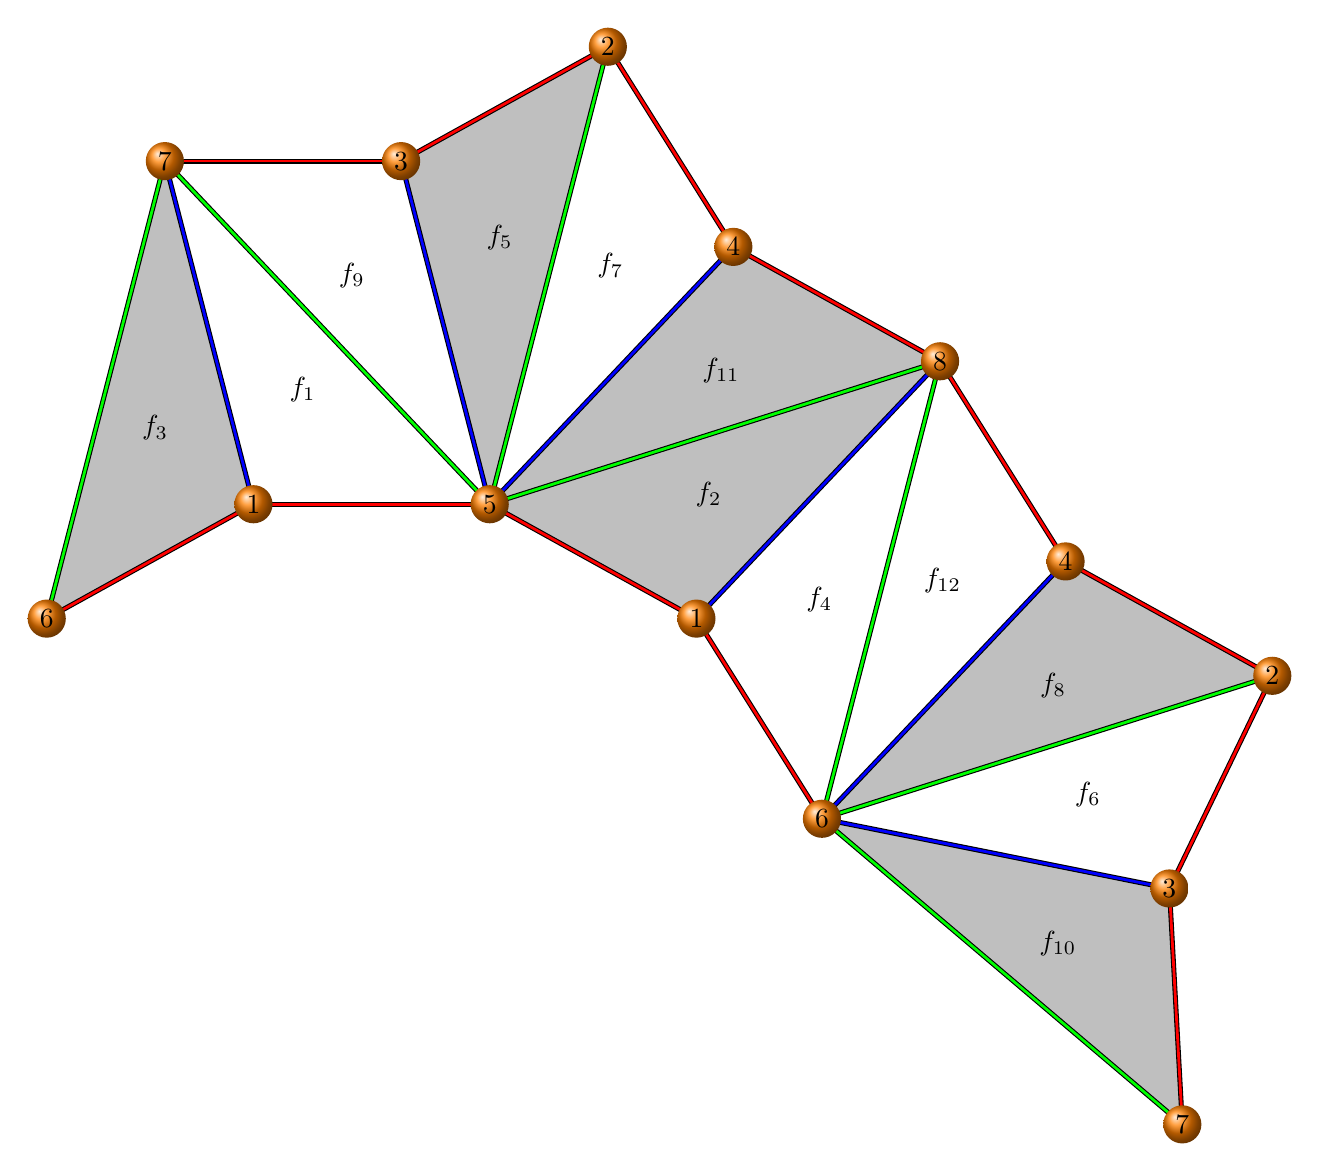
\begin{tikzpicture}[scale=3/2]
\coordinate (V1_1) at (0, 0);
\coordinate (V1_2) at (3.75, -0.9682458365518543);
\coordinate (V2_1) at (3, 3.872983346207417);
\coordinate (V2_2) at (8.625, -1.452368754827782);
\coordinate (V3_1) at (1.25, 2.904737509655563);
\coordinate (V3_2) at (7.75390625, -3.252700857166386);
\coordinate (V4_1) at (4.0625, 2.178553132241672);
\coordinate (V4_2) at (6.875, -0.4841229182759275);
\coordinate (V5_1) at (2, 0);
\coordinate (V6_1) at (-1.75, -0.9682458365518543);
\coordinate (V6_2) at (4.8125, -2.662676050517599);
\coordinate (V7_1) at (-0.75, 2.904737509655563);
\coordinate (V7_2) at (7.86328125, -5.249707895054585);
\coordinate (V8_1) at (5.8125, 1.210307295689818);


\fill[white] (V1_1) -- (V5_1) -- (V7_1) -- cycle;
\node (F1) at (0.4166666666666666, 0.9682458365518543) {$f_{1}$};
\fill[lightgray] (V1_2) -- (V5_1) -- (V8_1) -- cycle;
\node (F2) at (3.854166666666667, 0.08068715304598775) {$f_{2}$};
\fill[lightgray] (V1_1) -- (V6_1) -- (V7_1) -- cycle;
\node (F3) at (-0.8333333333333333, 0.6454972243679029) {$f_{3}$};
\fill[white] (V1_2) -- (V6_2) -- (V8_1) -- cycle;
\node (F4) at (4.791666666666666, -0.8068715304598785) {$f_{4}$};
\fill[lightgray] (V2_1) -- (V3_1) -- (V5_1) -- cycle;
\node (F5) at (2.083333333333333, 2.25924028528766) {$f_{5}$};
\fill[white] (V2_2) -- (V3_2) -- (V6_2) -- cycle;
\node (F6) at (7.063802083333333, -2.455915220837255) {$f_{6}$};
\fill[white] (V2_1) -- (V4_1) -- (V5_1) -- cycle;
\node (F7) at (3.020833333333333, 2.017178826149696) {$f_{7}$};
\fill[lightgray] (V2_2) -- (V4_2) -- (V6_2) -- cycle;
\node (F8) at (6.770833333333333, -1.533055907873769) {$f_{8}$};
\fill[white] (V3_1) -- (V5_1) -- (V7_1) -- cycle;
\node (F9) at (0.8333333333333333, 1.936491673103709) {$f_{9}$};
\fill[lightgray] (V3_2) -- (V6_2) -- (V7_2) -- cycle;
\node (F10) at (6.809895833333333, -3.72169493424619) {$f_{10}$};
\fill[lightgray] (V4_1) -- (V5_1) -- (V8_1) -- cycle;
\node (F11) at (3.958333333333333, 1.12962014264383) {$f_{11}$};
\fill[white] (V4_2) -- (V6_2) -- (V8_1) -- cycle;
\node (F12) at (5.833333333333333, -0.645497224367903) {$f_{12}$};


\tikzset{EdgeStyle/.style = {thin, double distance=1pt} }

\draw[ EdgeStyle, double=red] (V5_1) -- (V1_1);
\draw[ EdgeStyle, double=red] (V1_2) -- (V5_1);
\draw[ EdgeStyle, double=red] (V1_1) -- (V6_1);
\draw[ EdgeStyle, double=red] (V6_2) -- (V1_2);
\draw[ EdgeStyle, double=blue] (V1_1) -- (V7_1);
\draw[ EdgeStyle, double=blue] (V8_1) -- (V1_2);
\draw[ EdgeStyle, double=red] (V3_1) -- (V2_1);
\draw[ EdgeStyle, double=red] (V2_2) -- (V3_2);
\draw[ EdgeStyle, double=red] (V2_1) -- (V4_1);
\draw[ EdgeStyle, double=red] (V4_2) -- (V2_2);
\draw[ EdgeStyle, double=green] (V2_1) -- (V5_1);
\draw[ EdgeStyle, double=green] (V2_2) -- (V6_2);
\draw[ EdgeStyle, double=blue] (V3_1) -- (V5_1);
\draw[ EdgeStyle, double=blue] (V3_2) -- (V6_2);
\draw[ EdgeStyle, double=red] (V7_1) -- (V3_1);
\draw[ EdgeStyle, double=red] (V3_2) -- (V7_2);
\draw[ EdgeStyle, double=blue] (V4_1) -- (V5_1);
\draw[ EdgeStyle, double=blue] (V4_2) -- (V6_2);
\draw[ EdgeStyle, double=red] (V4_1) -- (V8_1);
\draw[ EdgeStyle, double=red] (V8_1) -- (V4_2);
\draw[ EdgeStyle, double=green] (V7_1) -- (V5_1);
\draw[ EdgeStyle, double=green] (V8_1) -- (V5_1);
\draw[ EdgeStyle, double=green] (V6_1) -- (V7_1);
\draw[ EdgeStyle, double=green] (V7_2) -- (V6_2);
\draw[ EdgeStyle, double=green] (V8_1) -- (V6_2);



\tikzset{VertexStyle/.style = {
 shape = circle,
 ball color = orange,
 text = black,
 inner sep = 2pt,
 outer sep = 0pt,
 minimum size = 10pt} }

\node[VertexStyle] at (V1_1) {1};
\node[VertexStyle] at (V1_2) {1};
\node[VertexStyle] at (V2_1) {2};
\node[VertexStyle] at (V2_2) {2};
\node[VertexStyle] at (V3_1) {3};
\node[VertexStyle] at (V3_2) {3};
\node[VertexStyle] at (V4_1) {4};
\node[VertexStyle] at (V4_2) {4};
\node[VertexStyle] at (V5_1) {5};
\node[VertexStyle] at (V6_1) {6};
\node[VertexStyle] at (V6_2) {6};
\node[VertexStyle] at (V7_1) {7};
\node[VertexStyle] at (V7_2) {7};
\node[VertexStyle] at (V8_1) {8};

\end{tikzpicture}

\end{document} 
